\chapter{Processors: Three-Loop, Third-Order Systems (3-OS)}\label{lect4}
\localtoc


In this chapter we will  close the third loop. It can be closed through a combinational circuit, through a memory circuit, or through an automaton. For our purpose, we are interested only on this last case, that of closing the third loop over an automaton through another automaton. We will focus, but not limited  on the third loop that allows us to introduce the concept of the processor exemplified with its simplest version, the {\bf {\em  elementary processor}}.  

We are also interested in investigating what the digital structure capable of recognizing or generating less restrictively generated languages ​​than regular ones, of type 3, looks like. Therefore, before describing the typical structure of three-loop systems, we will describe the minimal particular case that is associated with context-free languages.

\section{Counter-Expanded Automata and Context-Free Languages}

Let's remember how we solved the problem of recognizing strings of the form $1^n0^m$ using a finite automaton. What should we do if we try to recognize strings of the form $1^n0^n$, strings that have a higher complexity because we have an additional restriction: the number of 1s is the same as the number of 0s? A finite automaton, with a number of states independent of the value of $n$, cannot solve the problem. The solution is to add a reversible counter in the loop of a finite automaton. In Figure \ref{cea} a Counter-Expanded Automaton, CEA. It contains a reversible counter  that returns to the finite automaton  a flag indicating its zero state.

\placedrawing[h]{figures/F69.LP}{Counter-expanded automaton, CEA.}{cea}

Because both FA and UD/COUNTER are 2-OS, connecting them in loop results in having a 3-OS.

\begin{exemplu}\label{ceaEx}
The (context-free) language $(a^nb^n | \; n>0)$ is recognized by the  counter-expended automaton based on the following FA:
$$FA = ((X \times flag),(Y \times com),Q,f,g) =$$ 
$$= ((\{a,b,e\} \times \{zero\}), (\{idle, run, yes, no\} \times \{nop, up, down\}), Q, f, g)$$

\placedrawing[H]{figures/F70.lp}{The graph describing the behavior of the finite automaton used to build the counter-expanded automaton for the $(a^nb^n | \; n>0)$ language.}{ceaExGraph}

\hspace{-6mm}where $e$ is a delimiter symbol (a well-formed string is, for example, of the form $\ldots eeaaabbbee\ldots$),  and the set of states, $Q$, and the functions $f$ and $g$ are given by the graph in Figure \ref{ceaEx}. Establishing the  graph of the automaton allows us to also define the set of states: {\tt Q = \{q0, q1, q2, q3, q4\}}.

The top module for the System Verilog design is:
{\em
\includeverilogcode[caption={ Counter expanded automaton with a 32-bit counter for
             recognizing the language $a^nb^n$.  File: 0\_CEA.vh  (SystemVerilog)}, 
                    label={lst:CEA}, 
                    firstline=1, 
                    firstnumber=1, 
                    lastline=40]
                    {\verilogSourceDir/A11_CEA.sv}
}
\hspace{-6mm}while for the finite automaton FA the implementation is similar for the design in Example \ref{mealySV}.

$\diamond$
\end{exemplu}

Thus, after seeing that regular languages have finite automata as recognition and generation machines, we see that context-free languages have expanded automata with reversible counters as recognition and generation machines. In other words: type 3 languages correspond to two-loop systems -- ${\cal L}_3 \Leftrightarrow$ 3-OS -- and type 2 languages correspond to three-loop systems -- ${\cal L}_2 \Leftrightarrow$ 2-OS.


\section{Elementary Processor}

\subsection{Elementary Processor Structure}

The typical representative of 3rd order systems, 3-OS, is the elementary processor, EP.

\begin{definition}
An {\bf {\em elementary processor}} is obtained by loop connecting a functional simple automaton with a finite automaton used as controller in order to provide on output the result of a function applied on input data.

$\diamond$
\end{definition}
In Figure \ref{elemProc} the block schematic of an elementary processor, is represented. A standard implementation is with a RALU as the functional automaton (see \ref{rALU})  and a CROM as the control automaton(see \ref{contrAut}) . An EP performs a function specified on the input {\tt function}, which is applied to the data received on {\tt dataInput}. The result of the processing is provided on the output {\tt dataOutput}. The signals {\tt sync} are used to synchronize data transfer and function acknowledge.

\placedrawing[H]{figures/11_1_elementary_processor.LP}{Elementary Processor (EP) loop connecting a functional automaton, for example a RALU, with a control automaton, for example a CROM.}{elemProc}

The third loop is a control loop which sends commands from CROM to RALU, and sends back from RALU flags used by CROM to guide the evolution of the sequence of micro-instructions.

\begin{exemplu}\label{eProc}
Let us consider the EP whose top module is defined in Listing \ref{lst:elementaryProcessorEx}. The connections {\tt sync} are used to interact with the systems which provides {\tt dataInput} (input {\tt Ready} means {\tt dataInput} is valid and can be get by activating the output {\tt Read}) and receives {\tt dataOutput} (input {\tt Wait} means {\tt dataOutput} must be kept active until the system is able to get it). The hierarchy of modules describing the EP is the following:
\begin{itemize}
    \item {\tt 1\_elementaryProcessor.sv}:  is the top module formed by coupling the two automata, RALU  and CROM, in the third feedback loop 
    \begin{itemize}
        \item {\tt 2\_RALU.sv}:  is a simple functional automaton whose state is in the form of a Cartesian product that modifies at most one component per cycle under the command of the CROM unit
            \begin{itemize}
                \item {\tt 3\_regFile.sv}:  is the register file implemented as three-port memory from which we can read two states in each cycle, belonging to the Cartesian product of the states, and in which we can modify only one state per cycle
                \item {\tt 3\_ALU}:  is an arithmetic and logic units able to perform unary ans binary operations on values selected from the register file
            \end{itemize}
        \item {\tt 2\_CROM.sv}:  is a complex control automaton that can issue to the RALU unit sequences of commands (micro-instructions) initialized by the code applied to the input {\tt function}
            \begin{itemize}
                \item {\tt 3\_ROM.sv}:  stores a number of sequences of micro-instructions, called micro-programs that are selected from the {\tt function} input by the {\tt Init} command which is part of the {\tt sync} signals
            \end{itemize}
    \end{itemize}
\end{itemize}


{\em 
\includeverilogcode[caption={Example of Elementary Processor (EP).  File: 1\_elementaryProcessor.sv  (SystemVerilog)}, 
                    label={lst:elementaryProcessorEx}, 
                    firstline=1, 
                    firstnumber=1, 
                    lastline=100]
                    {\verilogSourceDir/A11_elementaryProcessor.sv}
}

The block schematic of the proposed elementary processor is represented in Figure \ref{fig:elementaryProcessor}. It is generated, starting from the description provided in Listing \ref{lst:elementaryProcessorEx}, by the Vivado toll.

\begin{figure}[H]
    \centering
    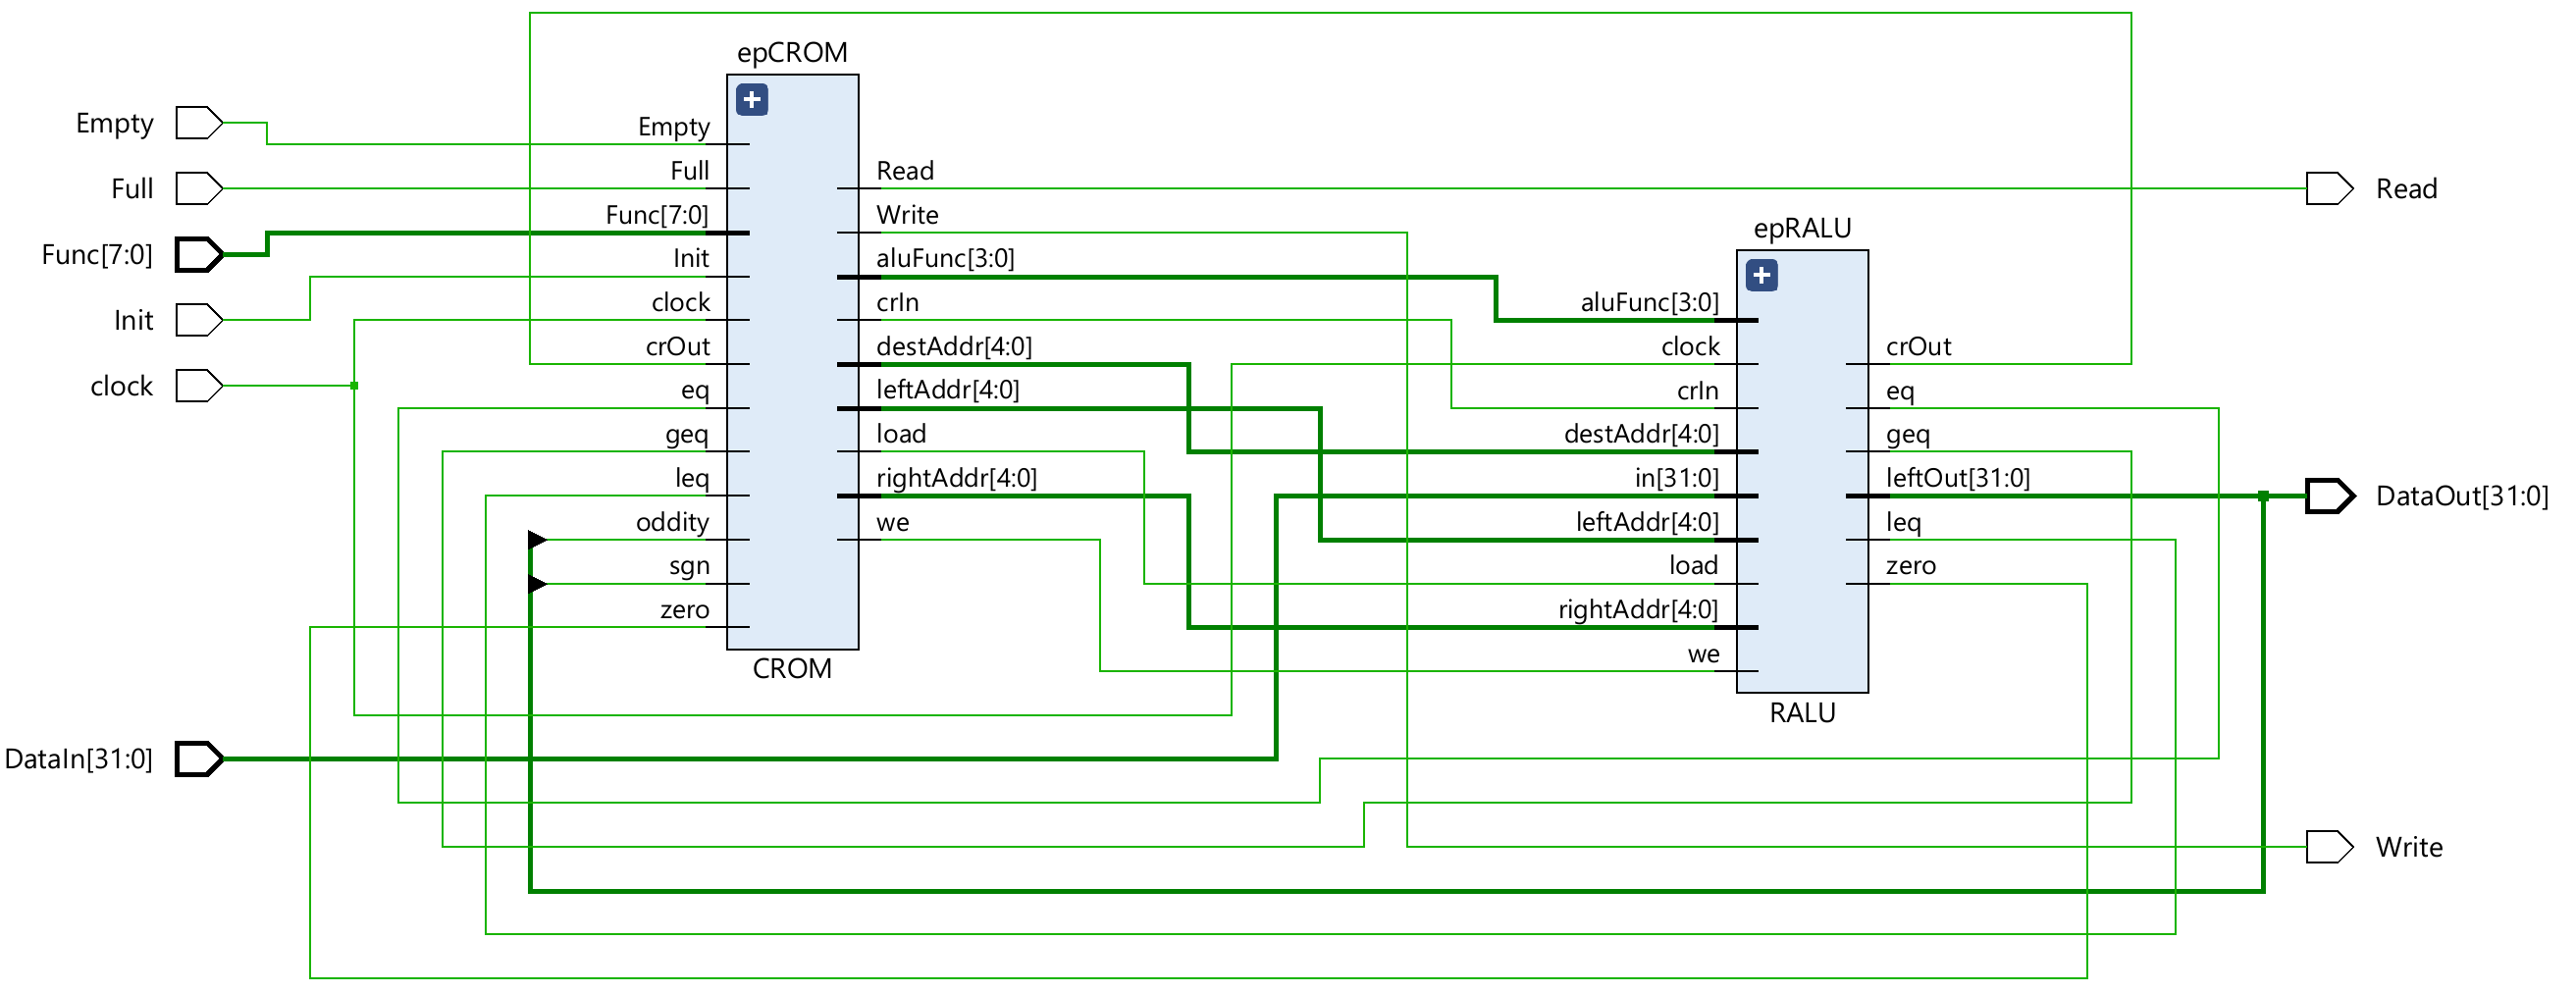
\includegraphics[width=\textwidth]{Images/elementaryProcessor.png} 
    \caption{Top level of the elementary processor generated in Vivado environment}
    \label{fig:elementaryProcessor}
\end{figure}

The simple functional automaton is a RALU, defined in Listing \ref{lst:elementaryProcessor}, unit with few additional simple circuits used to evaluate four flags besides the {\tt crOut} flag provided by the ALU output. They are evaluated on the two outputs of the register file, {\tt leftOut} and {\tt rightOut}, as follows: 

{\em 
\includeverilogcode[caption={RALU of Elementary Processor (EP).  File: 2\_RALU.sv  (SystemVerilog)}, 
                    label={lst:elementaryProcessor}, 
                    firstline=1, 
                    firstnumber=1, 
                    lastline=100]
                    {\verilogSourceDir/A11_RALU.sv}
}

\begin{figure}[H]
    \centering
    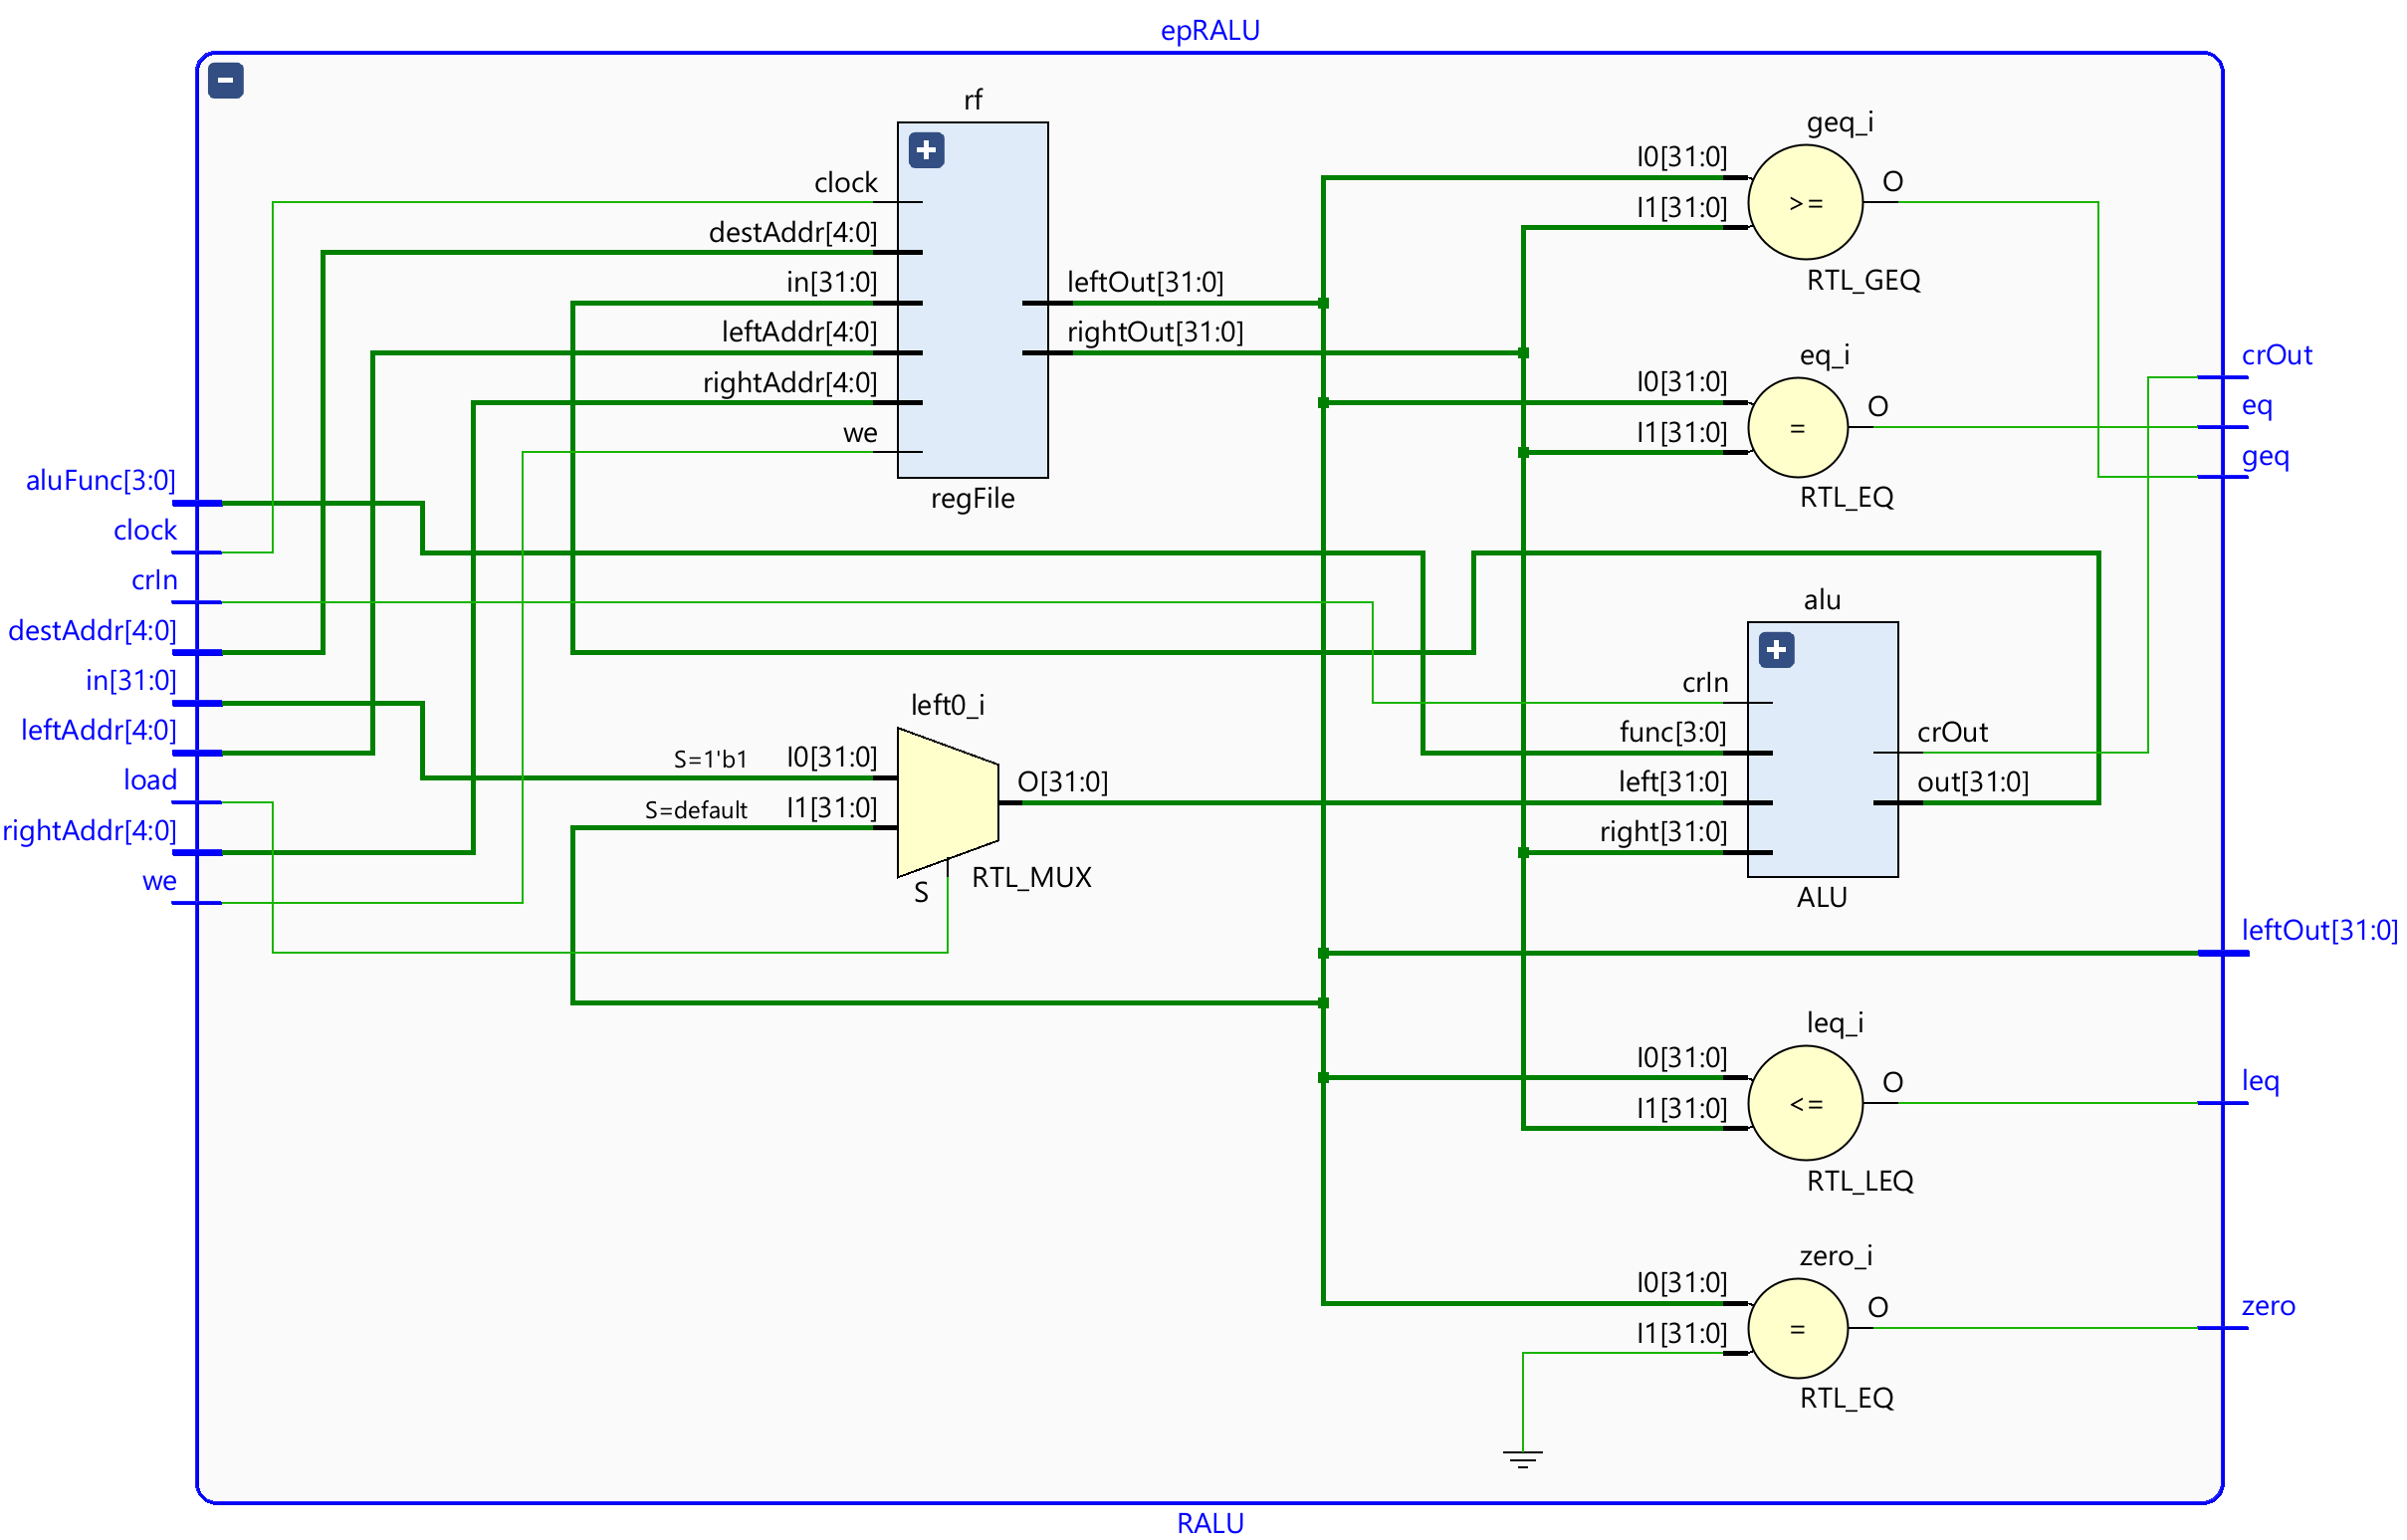
\includegraphics[width=\textwidth]{Images/peRALU.png} 
    \caption{epRALU.}
    \label{fig:peRALU}
\end{figure}

\begin{itemize}
    \item {\tt eq}: equal,  {\tt leftOut == rightOut}
    \item {\tt leq}: less than or equal, {\tt leftOut <= rightOut}
    \item {\tt geq}: greater than or equal, {\tt leftOut >= rightOut}
    \item {\tt zero}: equal with zero, {\tt leftOut == 0}
\end{itemize}
To these five flags two are added by directly selected them from the {\tt leftOut} output of the register file:
\begin{itemize}
    \item {\tt sgn}: indicates the number selected by {\tt L(v)} is negative
    \item {\tt oddity}: indicates the number selected by {\tt L(v)} is odd
\end{itemize}

The complex, control automaton CROM is described in Listing \ref{lst:CROM}, while de resulting structure is represented in Figure \ref{fig:epCROM} as it is generated by the Vivado tool. The complex part of the subsystem is concentrated in the content of the RAM combinational circuit. The rest of the CROM unit contains only simple circuits register, increment circuit and multiplexers.

To the flags provided by the RALU unit there are added two flags received from the external systems:
\begin{itemize}
    \item {\tt Empty}: the data source applied to the input {\tt DataIn} is empty, i.e., does not provide a valid data input for PE
    \item {\tt Full}: the data receiver is full, i.e., it is unable to take the data provided on {\tt DataOut} output of PE.
\end{itemize}

{\em 
\includeverilogcode[caption={CROM of Elementary Processor (EP).  File: 2\_CROM.sv  (SystemVerilog)}, 
                    label={lst:CROM}, 
                    firstline=1, 
                    firstnumber=1, 
                    lastline=100]
                    {\verilogSourceDir/A11_CROM.sv}
}

\begin{figure}[H]
    \centering
    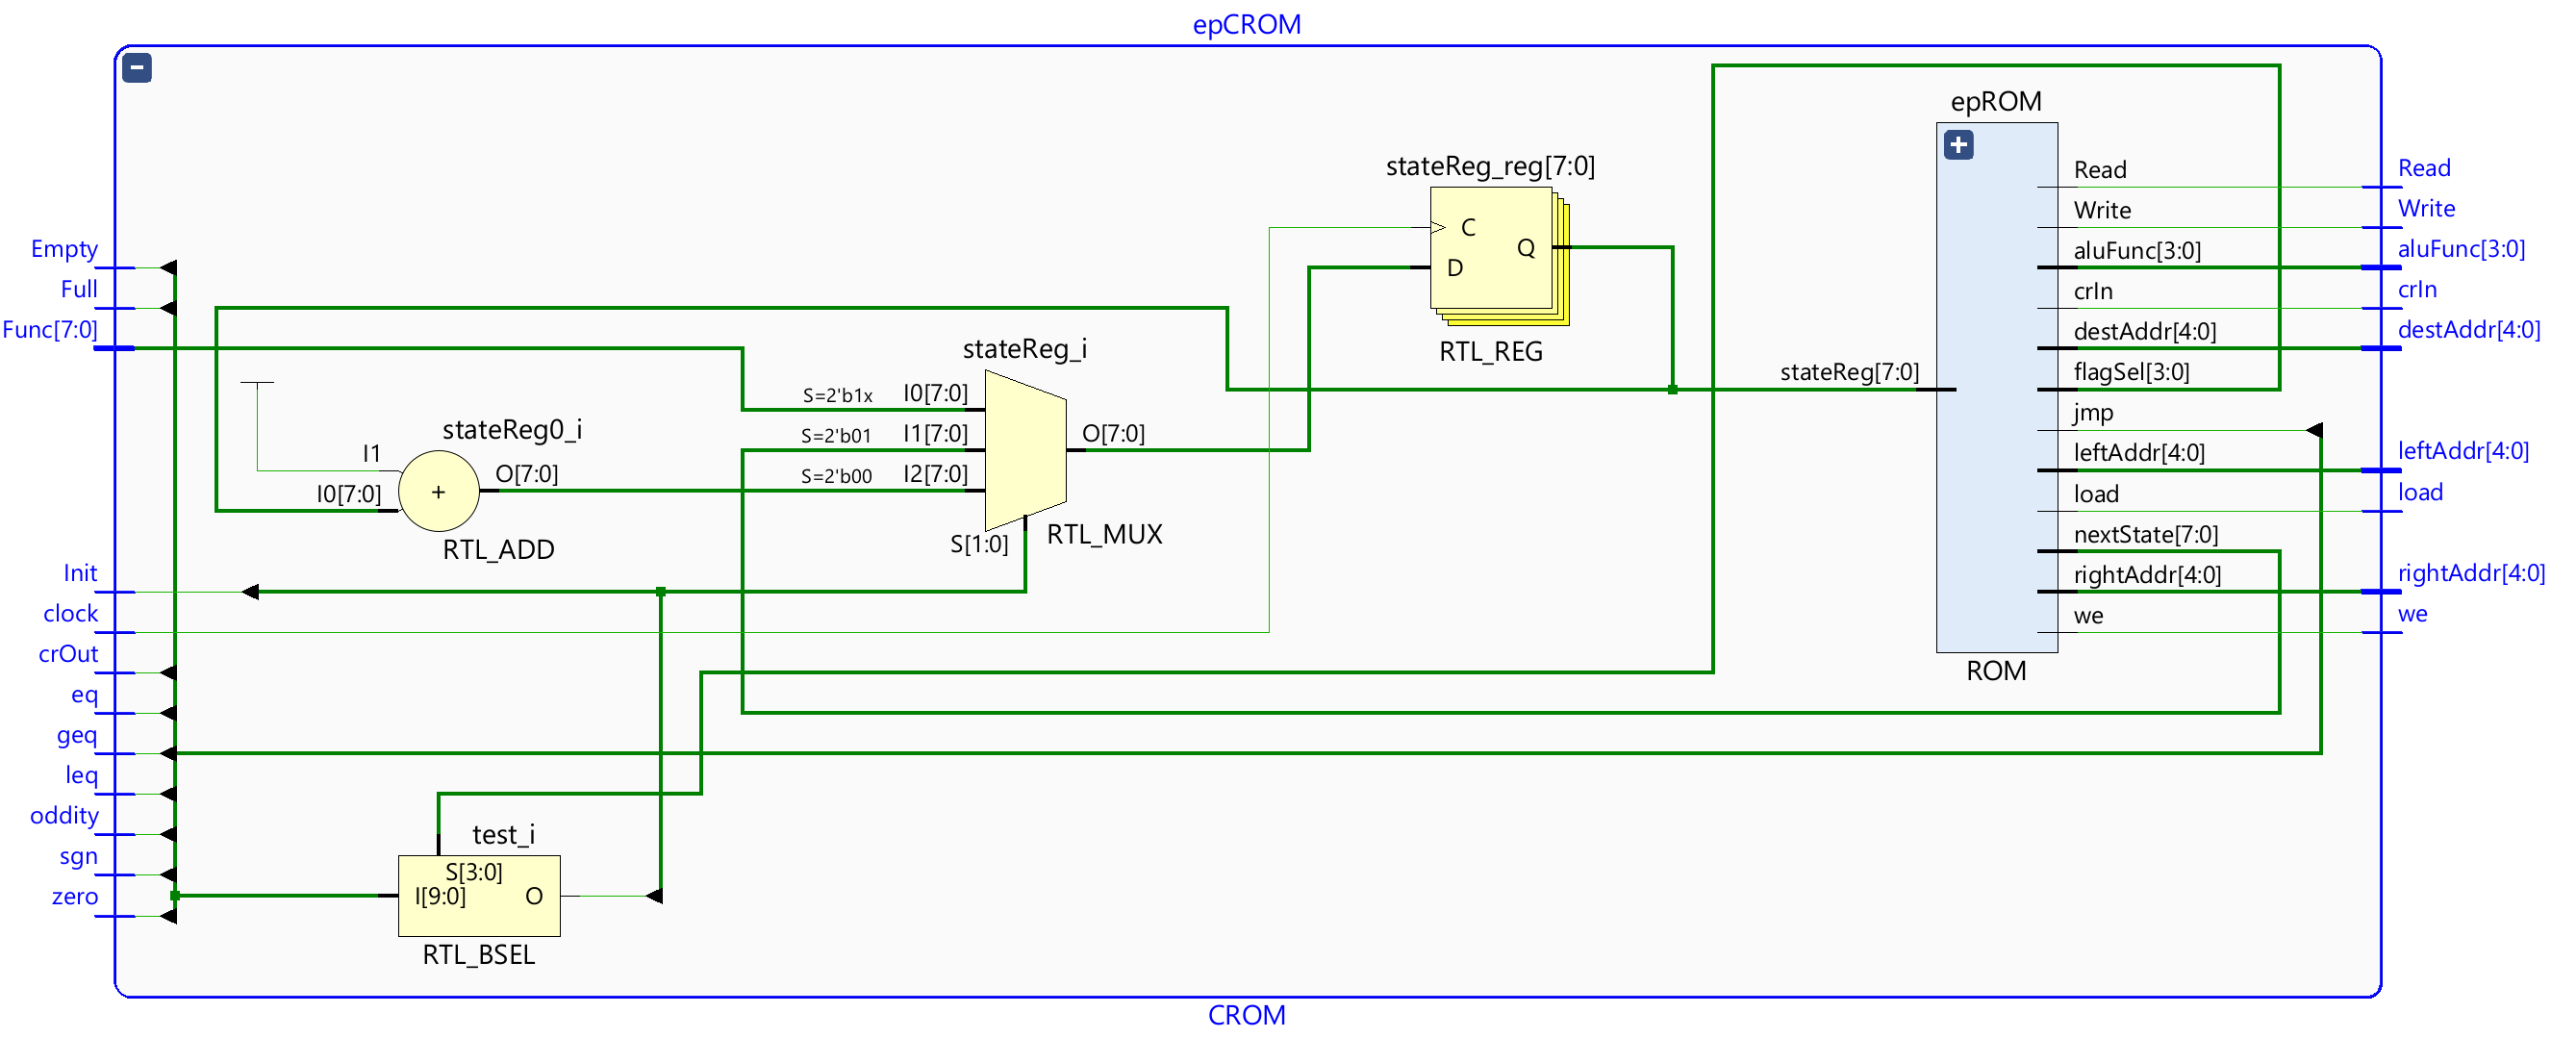
\includegraphics[width=\textwidth]{Images/epCROM.png} 
    \caption{epCROM.}
    \label{fig:epCROM}
\end{figure}

The third level of the design has two modules in RALU (register file and ALU) and one in CROM (the ROM circuit).

In Listing \ref{lst:regFile} the structure and function of the register file is designed, while the resulting schemaatic is presented in Figure \ref{fig:epRegFile}. The register file is a synchronous memory for writing and asynchronous for reading.

{\em 
\includeverilogcode[caption={Register file.  File: 3\_regFile.sv  (SystemVerilog)}, 
                    label={lst:regFile}, 
                    firstline=1, 
                    firstnumber=1, 
                    lastline=100]
                    {\verilogSourceDir/A11_regFile.sv}
}

\begin{figure}[H]
    \centering
    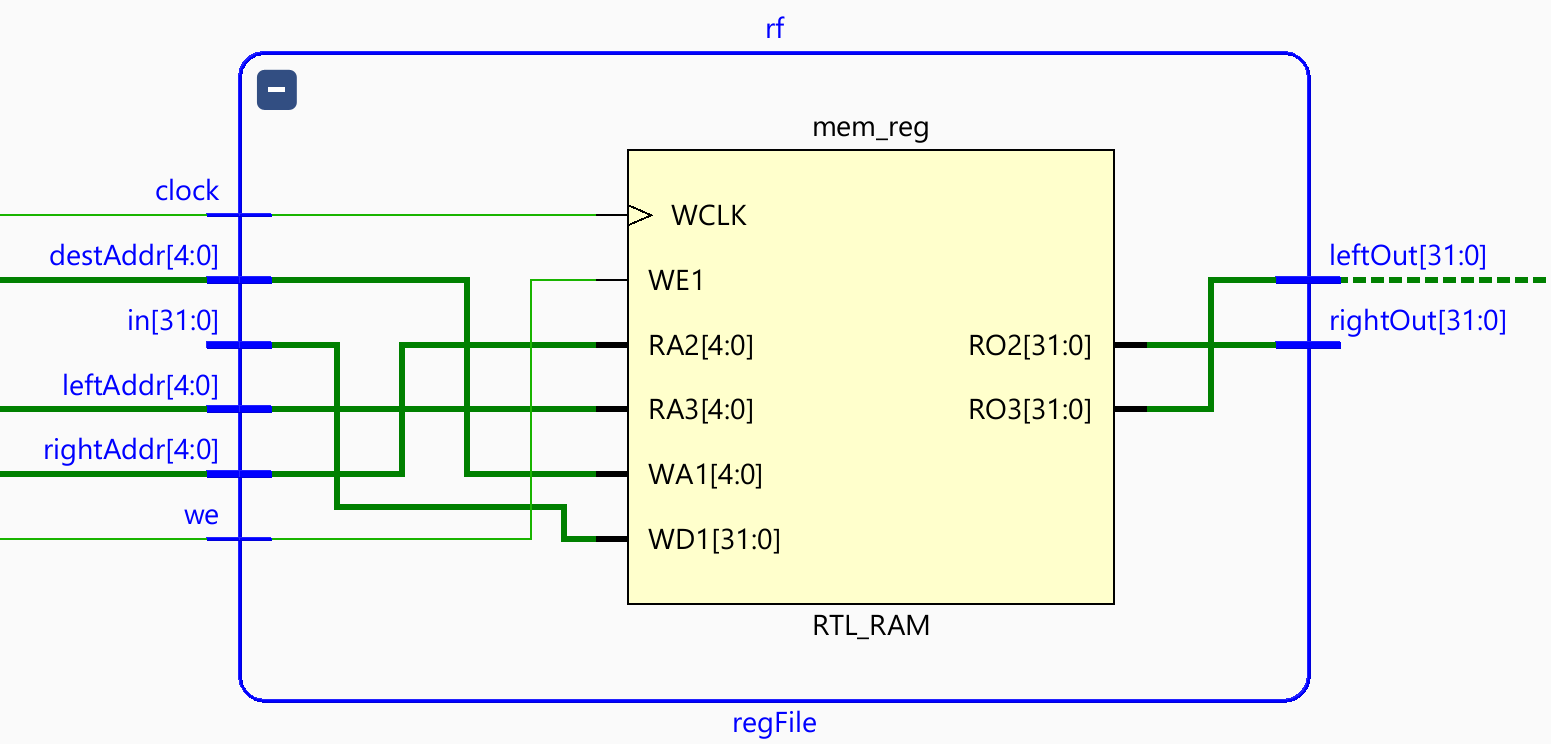
\includegraphics[width=\textwidth]{Images/epRegFile.png} 
    \caption{Register file.}
    \label{fig:epRegFile}
\end{figure}

In Listing \ref{lst:ALU} and Figure \ref{fig:epALU} the ALU used by the EP is described according to the {\tt 0\_define.vh} file (see Listing \ref{lst:define}).

{\em 
\includeverilogcode[caption={Define file for EP.  File: 0\_define.vh  (SystemVerilog)}, 
                    label={lst:define}, 
                    firstline=1, 
                    firstnumber=1, 
                    lastline=100]
                    {\verilogSourceDir/A11_define.vh}
}

\begin{figure}[H]
    \centering
    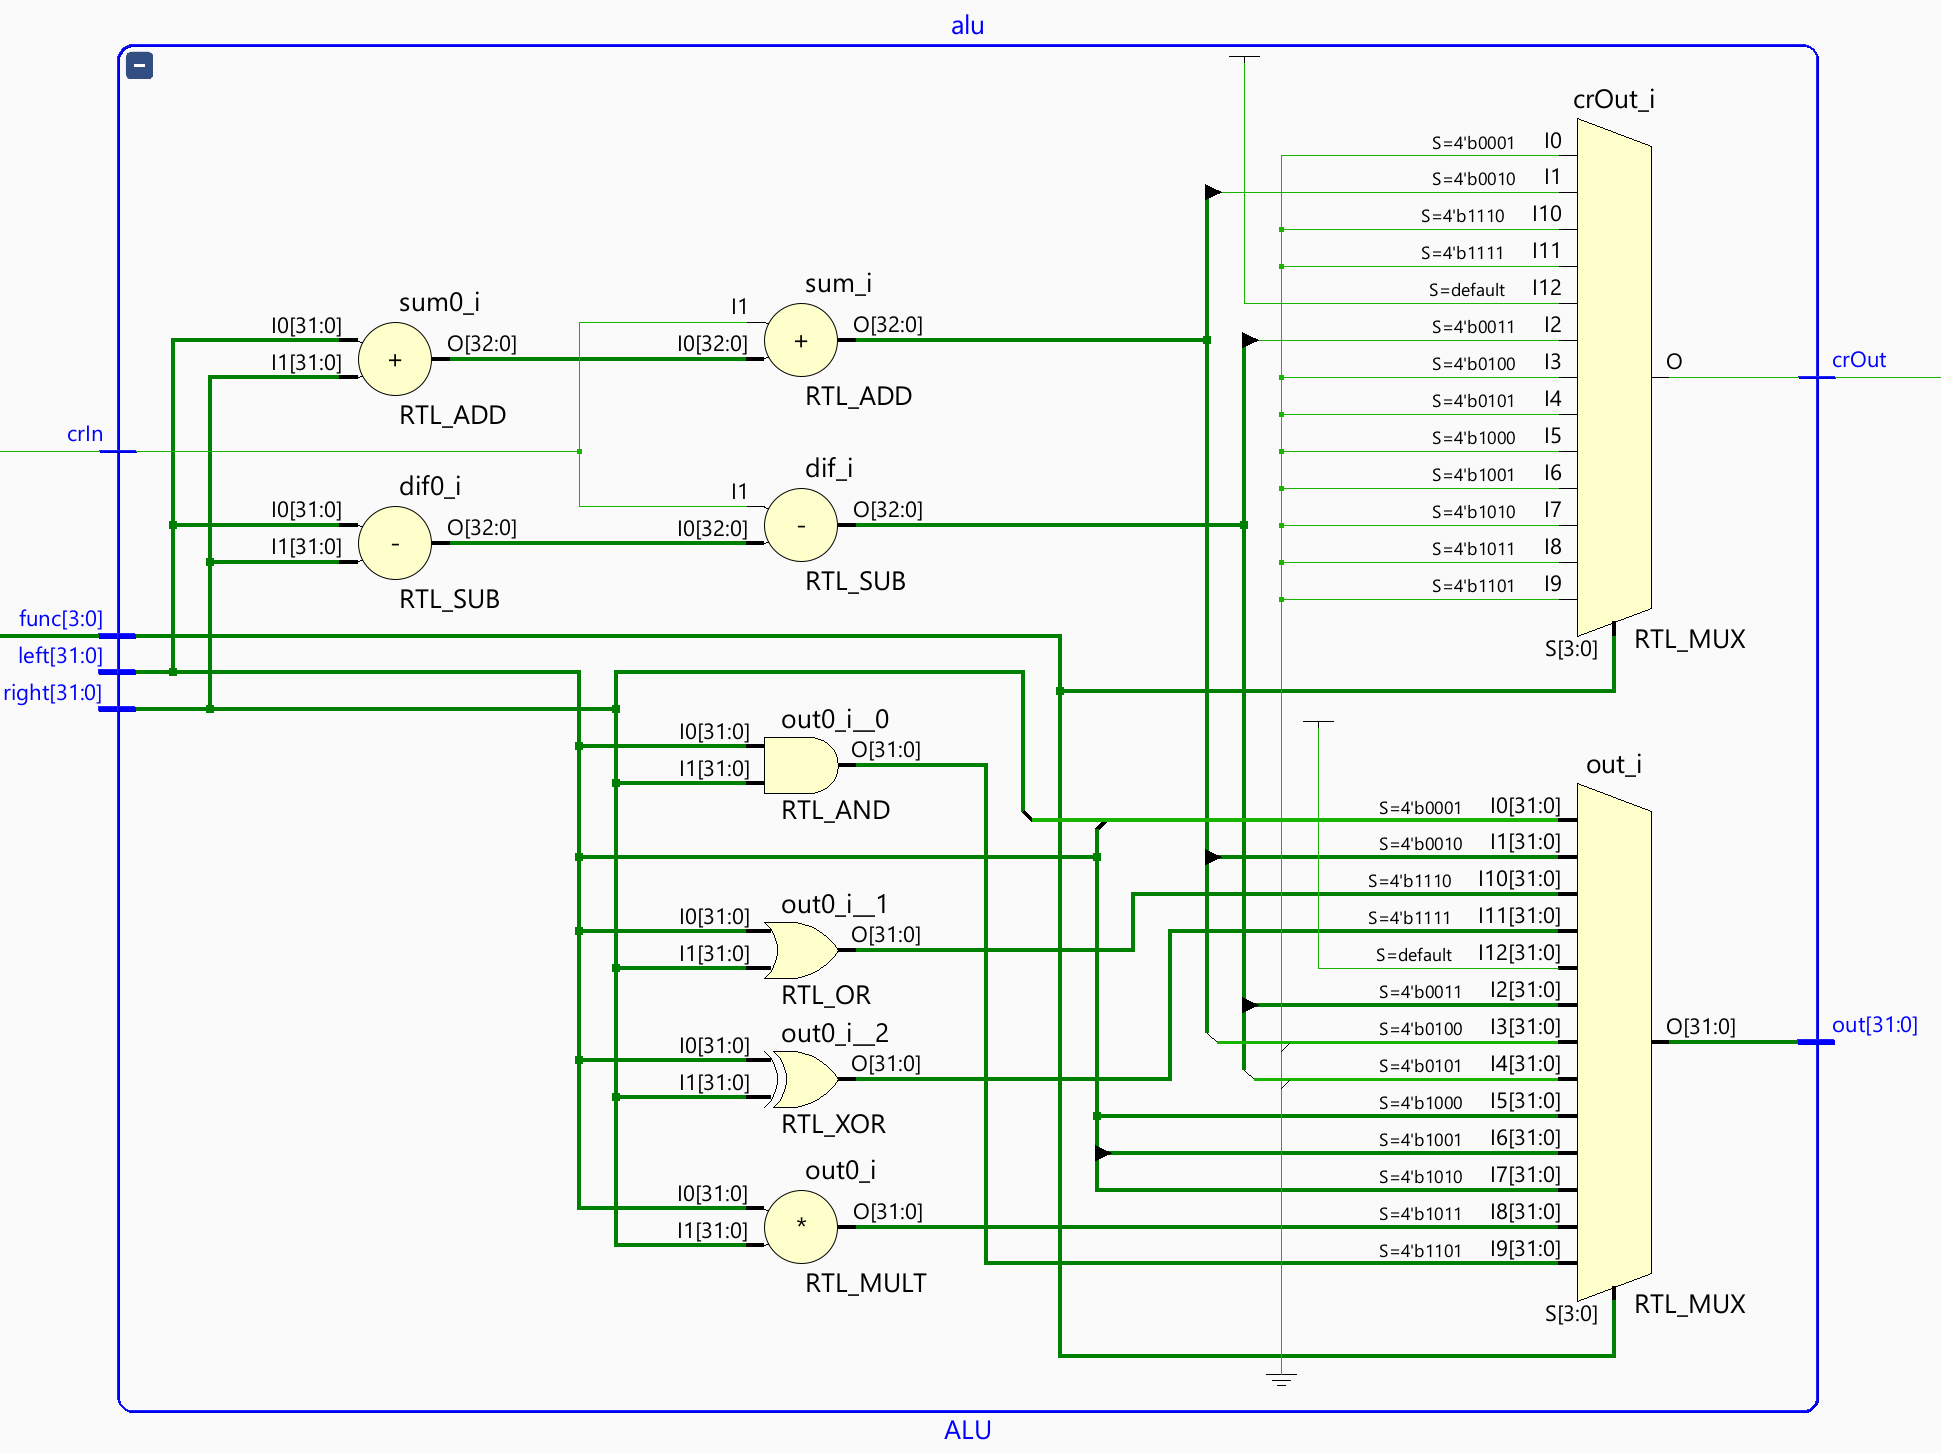
\includegraphics[width=\textwidth]{Images/epALU.png} 
    \caption{ALU.}
    \label{fig:epALU}
\end{figure}

{\em 
\includeverilogcode[caption={ALU.  File: 3\_ALU.sv  (SystemVerilog)}, 
                    label={lst:ALU}, 
                    firstline=1, 
                    firstnumber=1, 
                    lastline=100]
                    {\verilogSourceDir/A11_ALU.sv}
}

In Listing \ref{lst:ROM} and Figure \ref{fig:epROM} the ROM used by the CROM unit is structurally described. Its content is generated by {\tt \_microCodeGeneerator.sv} (see next subsection).

{\em 
\includeverilogcode[caption={epROM.  File: 3\_ROM.sv  (SystemVerilog)}, 
                    label={lst:ROM}, 
                    firstline=1, 
                    firstnumber=1, 
                    lastline=100]
                    {\verilogSourceDir/A11_ROM.sv}
}

\begin{figure}[H]
    \centering
    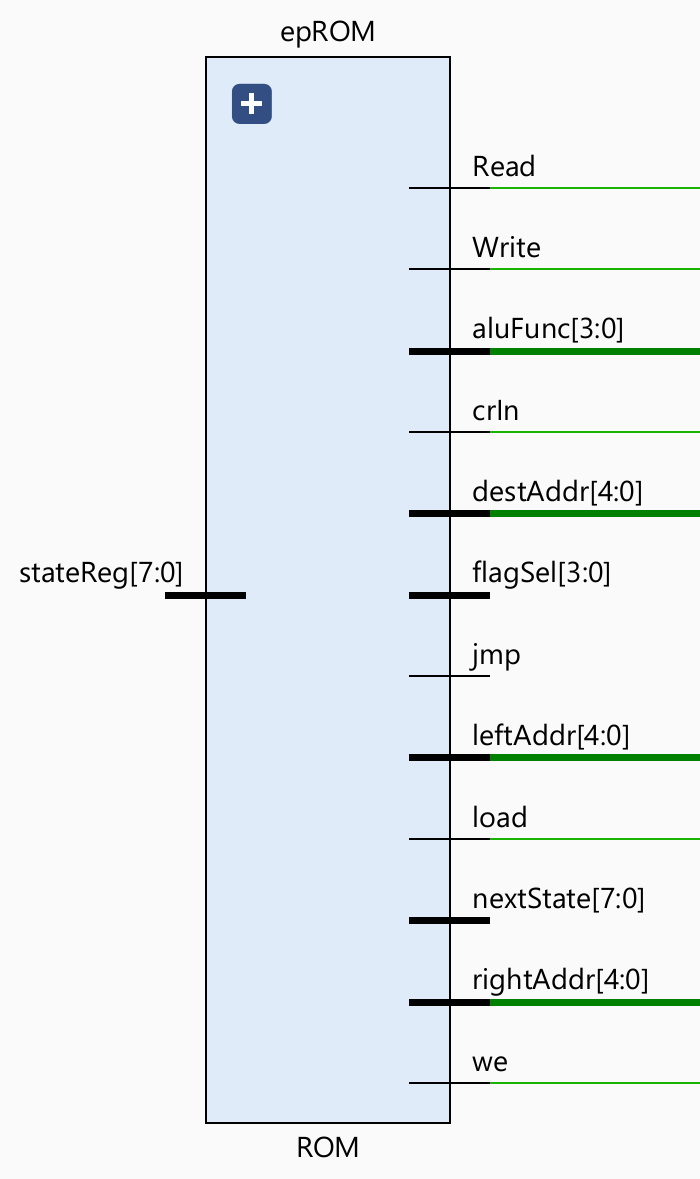
\includegraphics[width=6cm]{Images/epROM.png} 
    \caption{ROM.}
    \label{fig:epROM}
\end{figure}

$\diamond$
\end{exemplu}

\subsection{Elementary Processor Micro-Programming}

Micro-programming an EP means to establish the content of CROM's ROM. We must follow the next steps:
\begin{enumerate}
    \item define the fields of the output word of ROM
    \item define the meaning designate by each field
    \item design the program which generate the binary form of each word (line) in ROM
    \item write the micro-programs associated for each function
\end{enumerate}

\subsubsection{Micro-Program's Fields}

A micro-instruction is organized in fields, according to the command issued by the CROM unit. In Example \ref{eProc}, the micro-program uses micro-instructions with the following 12 fields:
\begin{description}
    \item[{\tt nextState[7:0]}]: represents the value of the next state when it is not determined by increment; is is specified in assembly language through the label associated to the targeted line, and the micro-code generator takes care about the actual binary value inserted in the micro-instruction
    \item[{\tt jmp}]: unconditioned jump to {\tt nextState} specified by label; it acts in micro-instruction with the following mnemonic:
        \begin{description}
            \item[{\bf  JMP(<label>)}]: where {\tt <label>} is expressed by a number
        \end{description}
    \item[{\tt flagSel[3:0]}]: selects the flag according to which the jump is made to  {\tt nextState}; it acts in micro-instruction with the followings mnemonics:
    \begin{description}
        \item[{\bf CRJMP(<label>)}]: jump, if carry, to {\tt <label>} which is expressed by a number
        \item[{\bf ODDJMP(<label>)}]: jump, if left operand is an odd number, to {\tt <label>} which is expressed by a number
        \item[{\bf SGNJMP(<label>)}]: jump, if left operand is a negative numbe,r  to {\tt <label>} which is expressed by a number
        \item[{\bf ZJMP(<label>)}]: jump, if left operand is zero,  to {\tt <label>} which is expressed by a number
        \item[{\bf LEQJMP(<label>)}]: jump, if left operand is less or equal than right operand,  to {\tt <label>} which is expressed by a number
        \item[{\bf GEQJMP(<label>)}]: jump, if left operand is greater or equal than right operand,  to {\tt <label>} which is expressed by a number
        \item[{\bf EQJMP(<label>)}]: jump, if left operand is  equal with right operand,  to {\tt <label>} which is expressed by a number
        \item[{\bf EMPTYJMP(<label>)}]: jump if the sender system is empty (has nothing to send), where {\tt <label>} is expressed by a number
        \item[{\bf FULLJMP(<label>)}]: jump is the receiver is full (unable to receive), where {\tt <label>} is expressed by a number
    \end{description}
    \item[{\tt leftAddr[4:0]}]: address to select the left operand for ALU from register file; it acts in micro-instruction with the following mnemonic:
        \begin{description}
            \item[{\bf L(<address>)}]: where {\tt <address>} is expressed by a number
        \end{description}
    \item[{\tt rightAddr[4:0]}]: address to select the right operand for ALU from register file; it acts in micro-instruction with the following mnemonic:
        \begin{description}
            \item[{\bf R(<address>)}]: where {\tt <address>} is expressed by a number
        \end{description}
    \item[{\tt crIn}]: carry input applied to ALU; it acts in micro-instruction with the following mnemonic:
        \begin{description}
            \item[{\bf CR}]
        \end{description}
    \item[{\tt destAddr[4:0]}]: address to select the destination of the result computed by ALU; it acts in micro-instruction with the following mnemonic:
        \begin{description}
            \item[{\bf D(<address>)}]: where {\tt <address>} is expressed by a number
        \end{description}
    \item[{\tt load}]: selects as left operand DataIn; it acts in micro-instruction with the following mnemonic:
        \begin{description}
            \item[{\bf LOAD}]
        \end{description}
    \item[{\tt we}]: write enable applied to the register file; it acts in micro-instruction with the following mnemonic:
        \begin{description}
            \item[{\bf WB}]:write back
        \end{description}
    \item[{\tt aluFunc[3:0]}]: the arithmetic or logic function selected to be performed by ALU on the operands fetched form the register file; it acts in micro-instruction with the followings mnemonics:
        \begin{description}
            \item[{\bf BIGVAL}]:
        \end{description}
        \begin{description}
            \item[{\bf ADD}]:
        \end{description}
        \begin{description}
            \item[{\bf SUB}]:
        \end{description}
        \begin{description}
            \item[{\bf ADDCR}]:
        \end{description}
        \begin{description}
            \item[{\bf SUBCR}]:
        \end{description}
        \begin{description}
            \item[{\bf LSH}]:
        \end{description}
        \begin{description}
            \item[{\bf ASH}]:
        \end{description}
        \begin{description}
            \item[{\bf MOVE}]:
        \end{description}
        \begin{description}
            \item[{\bf MULT}]:
        \end{description}
        \begin{description}
            \item[{\bf AND}]:
        \end{description}
        \begin{description}
            \item[{\bf OR}]:
        \end{description}
        \begin{description}
            \item[{\bf XOR}]:
        \end{description}
    \item[{\tt Read}]: read DataIn; it acts in micro-instruction with the following mnemonic:
        \begin{description}
            \item[{\bf GET}]
        \end{description}
    \item[{\tt Write}]: write DataOut; it acts in micro-instruction with the following mnemonic:
        \begin{description}
            \item[{\bf SEND}]
        \end{description}
\end{description}

\subsubsection{Writing a micro-program}

A line of micro-code contains 37 bits. Each line is "stored" in a single location of the ROM in CROM. We used quotation marks because ROM is not a memory and its content is not stored, it is imprinted using a technological procedure. 

The micro-instruction is organized in fields as follows:
{\small
\begin{verbatim}
{jmp,nextState,flagSel,leftAddr,rightAddr,crIn,destAddr,load,we,aluFunc,read,write}
\end{verbatim}
}
Each line in a micro-program must by specified only by the fields with active forms. All the other fields will remain specified by zeroes. For example, the micro-instruction which moves the content of a register from the register file in other register, must specify, in any order, only the values for the fields {\tt destAddr, leftAddr, aluFunc,} and {\tt we}. All the other fields will be set to the default value which is zero.

\begin{exemplu}\label{mcex}
Let be a micro-program initialized by loading in registers three values received from the data input. Then operate on the received data running a loop {\tt rf[6]+1} times starting at the label {\tt LB(0)} and ending in halt at the label {\tt LB(55)}. The micro-program considers that the input signals {\tt Empty} and {\tt Full} are inactive (the sender sends data and the receiver accepts data).
{\em 
\includeverilogcode[caption={Example of micro-program.  File: 0\_microProgram.sv  (SystemVerilog)}, 
                    label={lst:microProgram}, 
                    firstline=1, 
                    firstnumber=1, 
                    lastline=200]
                    {\verilogSourceDir/A11_microProgram.sv}
}

Each line ends with {\tt LL}, the command used by the micro-code generator to {\bf l}oads the {\bf l}ine in ROM. This command allows avoiding to specifiy for each line all the fields.

$\diamond$
\end{exemplu}


\subsubsection{Micro-Code Generator}

The simulator will be described in \ref{elProcSim} the following code is included. It will receive the file {\tt 0\_microProgram.sv} to be translated into binary form.

\includeverilogcode[caption={Micro-code generator.  File: 0\_microCodeGenerator.sv  (SystemVerilog)}, 
                    label={lst:microCodeGenerator}, 
                    firstline=1, 
                    firstnumber=1, 
                    lastline=200]
                    {\verilogSourceDir/A11_microCodeGenerator.sv}

\begin{verisum}{\em :

\hspace{-0.8cm} \rule[5mm]{16cm}{0.25mm} \vspace{-0.7cm}

\begin{description}
    \item[function] functionName; {\bf input} [...:...] inputName; ... {\bf begin} functionBody {\bf end  endfunction} : describes the function {\tt functionName} of parameters {\tt inputName} ... which performs the actions defined by {\tt functionBody}.
\end{description}
\rule[5mm]{16cm}{0.25mm} }
\end{verisum}

\begin{exemplu}
The micro-program from Example \ref{mcex} is translated in the following binary form using {\tt  0\_microCodeGenerator.sv} in the simulation module described in \ref{{elProcSim}}.

\begin{verbatim}
epROM[0]     = 0000000000000000000000000000011101000
epROM[1]     = 0000000000000000000000000010111101000
epROM[2]     = 0000000000000000000000000011011101000
epROM[3]     = 0000000000000000000000000000101001000
epROM[4]     = 0000000000000000010000100001001001000
epROM[5]     = 0000000000000000100001000001101001000
epROM[6]     = 0000000000000000110000000000001101000
epROM[7]     = 0000010010100001100010100011001001100
epROM[8]     = 1000000110000000000000000000000000000
epROM[9]     = 1000010010000000000000000000000000000
epROM[10]    = xxxxxxxxxxxxxxxxxxxxxxxxxxxxxxxxxxxxx
\end{verbatim}

$\diamond$
\end{exemplu}

\subsubsection{Elementary Processor Simulation}\label{elProcSim}

To test the operation of the elementary processor, we use the module in Listing \ref{lst:epTest} which generates the binary code of the micro-program and provides the external stimuli ({\tt clock, Inint, Func, DataIn, empty, Full}) for running the micro-program.

\includeverilogcode[caption={EP tester.  File: 0\_epTest.sv  (SystemVerilog)}, 
                    label={lst:epTest}, 
                    firstline=1, 
                    firstnumber=1, 
                    lastline=200]
                    {\verilogSourceDir/A11_epTest.sv}

\begin{exemplu}
The micro-program in Listing  \ref{lst:microProgram}  from Example \ref{mcex} works in conjunction with the stimulus generated by the simulation environment. Lines of code from 34 to 443 in Listing \ref{lst:epTest} provide the context for running the micro-program in Listing  \ref{lst:microProgram}. Results:
{\small
\begin{verbatim}
t=0  Func=0 Init=1 stateReg=x DataOut=x    test=x RF=[x x x x x x x x x]
t=1  Func=0 Init=1 stateReg=0 DataOut=x    test=0 RF=[x x x x x x x x x]
t=2  Func=0 Init=0 stateReg=0 DataOut=x    test=0 RF=[x x x x x x x x x]
t=3  Func=0 Init=0 stateReg=1 DataOut=3    test=0 RF=[3 x x x x x x x x]
t=5  Func=0 Init=0 stateReg=2 DataOut=3    test=0 RF=[3 x x x x 1 x x x]
t=7  Func=0 Init=0 stateReg=3 DataOut=3    test=0 RF=[3 x x x x 1 2 x x]
t=9  Func=0 Init=0 stateReg=4 DataOut=6    test=0 RF=[3 6 x x x 1 2 x x]
t=11 Func=0 Init=0 stateReg=5 DataOut=12   test=0 RF=[3 6 12 x x 1 2 x x]
t=13 Func=0 Init=0 stateReg=6 DataOut=24   test=0 RF=[3 6 12 24 x 1 2 x x]
t=15 Func=0 Init=0 stateReg=7 DataOut=2    test=0 RF=[24 6 12 24 x 1 2 x x]
t=17 Func=0 Init=0 stateReg=8 DataOut=24   test=1 RF=[24 6 12 24 x 1 1 x x]
t=19 Func=0 Init=0 stateReg=3 DataOut=24   test=0 RF=[24 6 12 24 x 1 1 x x]
t=21 Func=0 Init=0 stateReg=4 DataOut=48   test=0 RF=[24 48 12 24 x 1 1 x x]
t=23 Func=0 Init=0 stateReg=5 DataOut=96   test=0 RF=[24 48 96 24 x 1 1 x x]
t=25 Func=0 Init=0 stateReg=6 DataOut=192  test=0 RF=[24 48 96 192 x 1 1 x x]
t=27 Func=0 Init=0 stateReg=7 DataOut=1    test=0 RF=[192 48 96 192 x 1 1 x x]
t=29 Func=0 Init=0 stateReg=8 DataOut=192  test=1 RF=[192 48 96 192 x 1 0 x x]
t=31 Func=0 Init=0 stateReg=3 DataOut=192  test=0 RF=[192 48 96 192 x 1 0 x x]
t=33 Func=0 Init=0 stateReg=4 DataOut=384  test=0 RF=[192 384 96 192 x 1 0 x x]
t=35 Func=0 Init=0 stateReg=5 DataOut=768  test=0 RF=[192 384 768 192 x 1 0 x x]
t=37 Func=0 Init=0 stateReg=6 DataOut=1536 test=0 RF=[192 384 768 1536 x 1 0 x x]
t=39 Func=0 Init=0 stateReg=7 DataOut=0    test=1 RF=[1536 384 768 1536 x 1 0 x x]
t=41 Func=0 Init=0 stateReg=9 DataOut=1536 test=1 RF=[1536 384 768 1536 x 1 -1 x x]
\end{verbatim}
}

$\diamond$
\end{exemplu}



\section{Processor}\label{toyRISCprocessor}

The elementary processor defined above is capable of executing a single function using the microprogram written in the ROM associated with the CROM. If we call this single function an instruction, then it would be interesting if we could extend the functionality of the elementary processor to that of a processor that can execute a sequence of instructions. Instead of "waiting" for the activation of the external signal {\tt Init}, the processor can manage to fetch from a memory, which is external to it, the next instruction every time the current one has been executed. Furthermore, a processor is equipped with the capability of fetching from an external memory the data that it decides to use, not only those made available by an external mechanism as in the case of the elementary processor.

The internal state of the processor is given by the Cartesian product represented by the contents of the register file. The evolution of the internal state of the processor, under the influence of the sequence of instructions it controls and the data it accesses in the external memory, as well as the effect of this evolution on the data in the external data memory, are controlled by the sequence of instructions designed to be stored in a memory external to the processor. Under these conditions, the operation of a processor is determined by its hardware structure and the software structure of the programs it runs. For this reason, the description of a processor involves the complementary processes of defining the organization and architecture.

\subsection{Architecture vs. Organization}\label{archOrg}

{\small
 \hfill{
\begin{minipage}{8cm}
{\em Architecture: describes what the processor does.

Organization: describes how it does it.}
\end{minipage}
}}

\bigskip
In the beginning it was only the hardware and the software. At some point there was a need for an interface that would provide the software with a more friendly development environment. What it is? If in a suite of hardware implementations the set of instructions changes radically with each new version, then the programs written for previous versions are thrown into the trash every time a new hardware version is instantiated. This bad habit is cured with the design, at the beginning of the 1960s, of the IBM System/360. At that moment it was decided that:
\begin{quote}
{\em ... to describe the
attributes of a system as seen by the programmer, i.e., the conceptual structure
and functional behavior, as distinct from the organization of the data flow and
controls, the logical design, and the physical implementation.} \citep{Amdahl64}
\end{quote}
And so the {\em Hardware -- Software} duet turned into the {\bf {\em Hardware -- Architecture -- Software}} triplet. Architecture being the short form for Instruction Set Architecture, ISA.
\begin{table}[H]
  \begin{center}
    \caption{Architecture vs. Organization.}
    \label{avso}
    {\small
    \begin{tabular}{|p{6cm}|p{6cm}|}
      \hline
     {\bf Architecture}                 & {\bf Organization}                                \\ \hline \hline
     describes what the processor does   & describes how it does it                          \\ \hline
     deals with the functional behavior & deals with a structural relationship              \\ \hline
     architecture is fixed first        & organization is decided after     \\ \hline
     comprises instruction sets, registers, data types, and addressing modes & consists of  multiplexers, adders, multipliers, peripherals, memories, ...\\ \hline
     the software developer is aware of it & it escapes the software programmer’s detection\\ \hline
    \end{tabular}
    }
  \end{center}
\end{table}


There are several ways to close the third loop over a generic 2-OS represented by an automaton in order to obtain the generic structure o a {\bf processor}. On the closed loop over an automaton we can connect a 0-OS (a combinational circuit), a 1-OS (a memory), or a 2-OS (an automaton). The last version is the most significant (see Figure \ref{fig40}). It is the main subject of this chapter.

The two machines that configure a processor have distinct functions:

\placedrawing[H]{figures/05_01_generic_processor.lp}{Generic processor: an engine capable of controlling the retrieval of data and instructions from the external memory source.}{fig40}

\begin{itemize}
    \item functional automaton that performs data processing functions; it is a simple automaton
    \item control automaton that ensures the sequential operation of the processor implemented in two possible versions:
        \begin{itemize}
            \item  a complex controller of the type presented in \ref{contrAut}, when, in addition to fetching the instruction from the program memory, it is also necessary to break it down into a sequence of micro-instructions executed by the functional automaton
            \item  a simple controller of the counter type presented in \ref{progCounter}, when it is sufficient to bring the instruction from the program memory because the instruction is simple enough to be executed directly by the functional automaton
        \end{itemize}
\end{itemize}

The two types of control generate two types of processors: interpreting processor and executing processor.

\subsection{Interpreting Processor (CISC processor)}

The first type of processor, the one that interprets the instruction by decomposing it into a sequence of microinstructions, is represented in Figure \ref{fig41}, where the control is performed with a complex automaton. An instruction can involve complex operations implemented sequentially through a series of micro-instructions sent by the controller to the functional automaton that can send back to the controller flags that can characterize the result of the application of each micro-instruction. For this reason, this processor version is called CISC (Complex Instruction Set Computer).

For each instruction the CISC processor must perform:
\begin{enumerate}
    \item instruction fetch
    \item instruction execute
    \item compute the address for the next instruction
\end{enumerate}

\placedrawing[H]{figures/05_02_interpreting_processor.lp}{Interpreting Processor}{fig41}

\hspace{-5mm}so that an instruction is executed in a variable number of at least several clock cycles.

\subsection{Executing Processor (RISC processor)}

The second type of processor is designed in such a way that it executes each instruction in constant time, usually one clock cycle, but no more than two clock cycles. Because each instruction requires fetching it from memory, and some instructions also require writing or reading data from memory, it is necessary to structure the memory into two sub-memories, one for programs and another for data. This results in the structure in Figure \ref{fig42}, where the processor has two access paths to memory resources.
In this case, the control automaton can only take care of fetching the instructions from the program memory and the functional automaton will execute sufficiently simple instructions to require only one clock cycle to be operated.

How did you get to this way of designing a processor that executes only simple, executable instructions in one clock cycle? Around 1980, the following facts were evident:

\placedrawing[H]{figures/05_03_executing_processor.lp}{Executing Processor}{fig42}

\begin{itemize}
    \item the frequency with which the instructions of a CISC processor appeared in the programs was very variable: a small number of instructions had a very high frequency of use, and the majority were used with low frequencies

    \item if the instructions were listed in descending order of frequency of use, then a line could be drawn in this list delimiting a set of frequently used instructions that also had the quality of being able to implement the instructions below the line through a suitable sequencing of them

    \item the pleasant surprise was that only simple functions were found above the line

    \item thus, for frequent operations, the effector structure could be imagined to work quickly, and for the less frequent ones, the possibility of their performance is ensured
\end{itemize}
Thus, a RISC processor executes instead of interpreting. Programs represent sequences of simple instructions, which are executed in parallel with the control of their evolution. Indeed, the functional automaton operates on the data while the control automaton calculates the address from which the next instruction will be read.
Both types of operations fall into the category of simple ones, the fact that it allows us to consider a RISC processor as simple to distinguish it from a CISC one which is complex due to the control automaton.

\bigskip

Since the functionality of a processor is exercised in the context of its use as a unit that runs a program stored in an external memory, we prefer to analyze in detail the functioning of a processor as part of a computing system. We will prefer to analyze in detail a RISC processor, an analysis that we will do in the context of a 5th order digital system (see Chapter \ref{lect6a}).


\section{Problems}

\subsection{Counter-Expanded Automata}

\begin{problem}
Design and simulate FA defined in Example \ref{ceaEx} by the graph represented in Figure \ref{ceaExGraph}.

$\diamond$
\end{problem}

\begin{problem}
Consider the language $L = \{a^nb^3c^4 \;| \; n>0\}$. Design the CEA which recognize this language. It is required:
\begin{enumerate}
    \item defining the graph which describes the associated finite automaton
    \item describing in System Verilog the CEA 
    \item verification of the design by simulation.
\end{enumerate}

$\diamond$
\end{problem}

\begin{problem}\label{pda}
Reconsider the structure defined in Example \ref{ceaEx} by substituting the up-down counter with the LIFO memory described in \ref{lb:lifo}. The initial top of stack must be a special symbol, $Z_0$. The resulting structure is called in literature: {\em push-down automaton}.

$\diamond$
\end{problem}


\begin{problem}
Use the push-down automaton designed in Problem \ref(pda) to solve the problem of recognizing $L = \{a^nc^4 \;| \; n>0\}$.

$\diamond$
\end{problem}

\subsection{Elementary Processor}

\begin{problem}
In Example \ref{mcex} the is considered {\tt Empty = 0} and {\tt Full = 0} during the test. Rewrite the micro-program considering that the two signals can take both the value 0 and the value 1 during the test. Test the correct functioning of the program using the Vivado environment and the simulator available on GitHub.

$\diamond$
\end{problem}

\begin{problem}
Modify the design of the elementary processor PE so that the new version, PE1, has the ability to generate, using CROM resources, constants that can be loaded into the register file.

$\diamond$
\end{problem}

\begin{problem}
Using PE1, design a  discrete-time FIR filter of order N, for $N=16$ taps, which receives a sting of integers, $x[i]$, and issues another string of integers, $y[j]$ according to the following expression:
$$y[n] = \sum_0^N b_ix[n-i]$$
The taps are generated in the definition of CROM.

$\diamond$
\end{problem}


